\documentclass[11pt]{article}
\usepackage[utf8]{inputenc}
\usepackage{geometry}
\usepackage{graphicx}
\usepackage{hyperref}
\usepackage{amsmath}
\usepackage{amsfonts}
\usepackage{amssymb}
\usepackage{color}
\usepackage[capitalise,noabbrev]{cleveref}
\usepackage{caption}
\usepackage{subcaption}
\usepackage[skip=14pt plus1pt, indent=0pt]{parskip}
\geometry{a4paper}
\usepackage{float}

\title{Cardano DEX Protocol with DIDs Layer}
\author{MuesliSwapTeam}
\date{\today}

\usepackage{biblatex}
\addbibresource{references.bib}


\begin{document}

\maketitle
\vspace{3em}

\begin{abstract} \noindent
In the evolving landscape of decentralized finance (DeFi), regulatory compliance and user trust remain paramount challenges. The MuesliSwap Team proposes an innovative approach to these challenges by extending the MuesliSwap Orderbook Decentralized Exchange (DEX) on the Cardano blockchain to include a governance framework leveraging Atala Prism's digital identity system. This report outlines the findings from the initial phase (Milestone 1) of the project, which focuses on research and design. Our objectives were to review the existing MuesliSwap DEX protocol, explore the capabilities of Atala Prism, and design an integration architecture that incorporates a decentralized identity (DID) layer for compliance without compromising the decentralized ethos of the platform.

\end{abstract}
\newpage 

\tableofcontents
\newpage

\section{Introduction}
Decentralized exchanges (DEXs) represent a critical component of the blockchain ecosystem, enabling peer-to-peer trading without the need for centralized intermediaries. The MuesliSwap Orderbook DEX on the Cardano blockchain exemplifies this innovation, offering a platform where users can trade digital assets directly and securely. However, as the DeFi space evolves, there's a growing need to enhance these platforms' efficiency, security, and regulatory compliance. This document introduces a pioneering project aimed at extending the MuesliSwap Orderbook DEX by incorporating the Atala PRISM Decentralized Identifier (DID) framework, a move designed to revolutionize user identity verification and compliance processes within the DEX environment.

The purpose of this document is to outline the research objectives and proposed solutions for the initial milestone of the project focused on extending the MuesliSwap DEX. This milestone concentrates on the thorough exploration and conceptualization of integrating Atala PRISM DID with the DEX infrastructure, aiming to provide a more secure, compliant, and user-friendly trading experience. Key areas of investigation include the seamless integration of DID technology for enhanced user verification, the implications of such integration on trading efficiency and regulatory adherence, and an extensive review of existing DEX solutions that could benefit from DID incorporation.

\paragraph{Scope and Structure.} The scope of this milestone is primarily research-oriented. The structure of this document is organized as follows:
\begin{itemize}
\item \textbf{Review of Existing DEX Orderbook:} This section will conduct a detailed analysis of our current orderbook DEX. This comprehensive review will help integrating the DID framework to meet the unique needs of decentralized trading platforms.

\item \textbf{Integration of Atala PRISM DID into the DEX:} This section will provide a conceptual overview of how Atala PRISM DID can be integrated into the existing DEX framework to enhance user identity verification processes. The goal is to increase security and privacy for users while simplifying compliance with regulatory requirements.
\item \textbf{Strategic Plan for DID Integration:} The document will conclude with a strategic roadmap for integrating Atala PRISM DID into the MuesliSwap DEX. This plan aims to outline the steps needed to achieve a seamless merger of DEX functionalities with the advanced identity verification features provided by DID technology.
\end{itemize}

By addressing these components, the document lays the groundwork for the next phases of development, ensuring a strategic and informed approach toward realizing the goal of enhancing the MuesliSwap Orderbook DEX with Atala PRISM DID. This initiative promises to set a new standard for security, efficiency, and compliance in the decentralized trading landscape.

\newpage

\section{The MuesliSwap Orderbook}

The MuesliSwap Decentralized Exchange (DEX) on the Cardano blockchain represents a significant milestone in the evolution of decentralized finance (DeFi), being the first to offer decentralized token swaps on this platform. Since its launch in November, 2021, MuesliSwap has been a testament to the possibilities and enthusiasm surrounding DeFi on Cardano. This section of the report delves into the technical workings of the MuesliSwap Orderbook DEX, aiming to demystify its operations for users and stakeholders alike.

\subsecection{Decentralized Orderbook Exchange Model}
Unlike many decentralized exchanges that adopt an Automated Market Maker (AMM) model, such as Uniswap on Ethereum, MuesliSwap employs a traditional order book model but in a decentralized fashion. This choice is deliberate, as discussed in our whitepaper, where we explore the benefits of such a model in the context of an EUTXO-based blockchain like Cardano. The order book model offers advantages in terms of concurrency, contention avoidance, fairness, and efficiency, making it an attractive option for a DEX on Cardano.

\subsection{Trading Workflow}
To illustrate the trading process on MuesliSwap, consider a user, Charles, who wishes to purchase 10 MILK tokens for no more than 5 ADA, setting a limit price of 0.5 ADA per MILK. Charles places his order through the MuesliSwap platform, which then locks his 5 ADA along with additional metadata in a smart contract on the Cardano blockchain. This action effectively registers Charles's interest in trading within the decentralized order book maintained on the blockchain (see \ref{fig:illustration1} for an illustration). 

\begin{figure}[H]
    \centering
    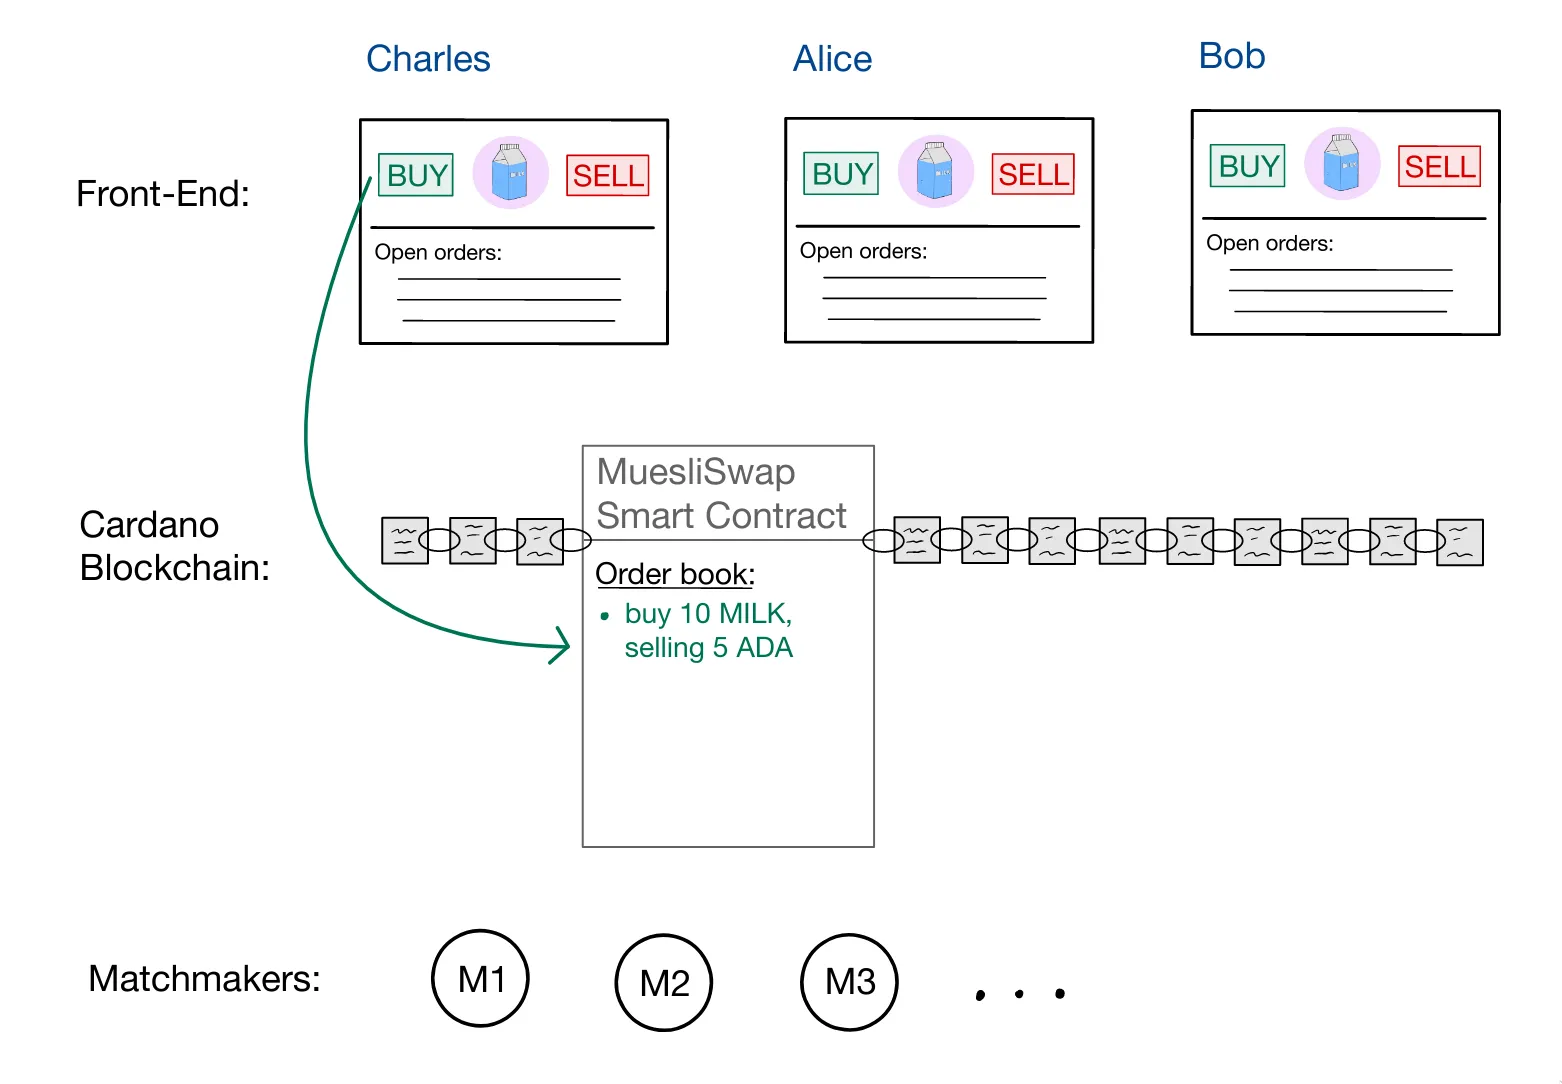
\includegraphics[scale=0.18]{illustration1.png}
    \caption{Charles placing an order of his beloved MILK by submitting it to the order book maintained by the MuesliSwap smart contract.}
    \label{fig:illustration1}
\end{figure}

Subsequently, other users, Alice and Bob, submit competing sell orders for MILK tokens at different prices. Alice asks for a minimum of 6 ADA for her 10 MILK tokens, while Bob is willing to accept 4 ADA for the same amount. These orders, along with Charles's, are entered into the MuesliSwap order book without involving any third-party intermediaries, highlighting the decentralized nature of the exchange. (see \ref{fig:illustration2} for an illustration).

\begin{figure}[H]
    \centering
    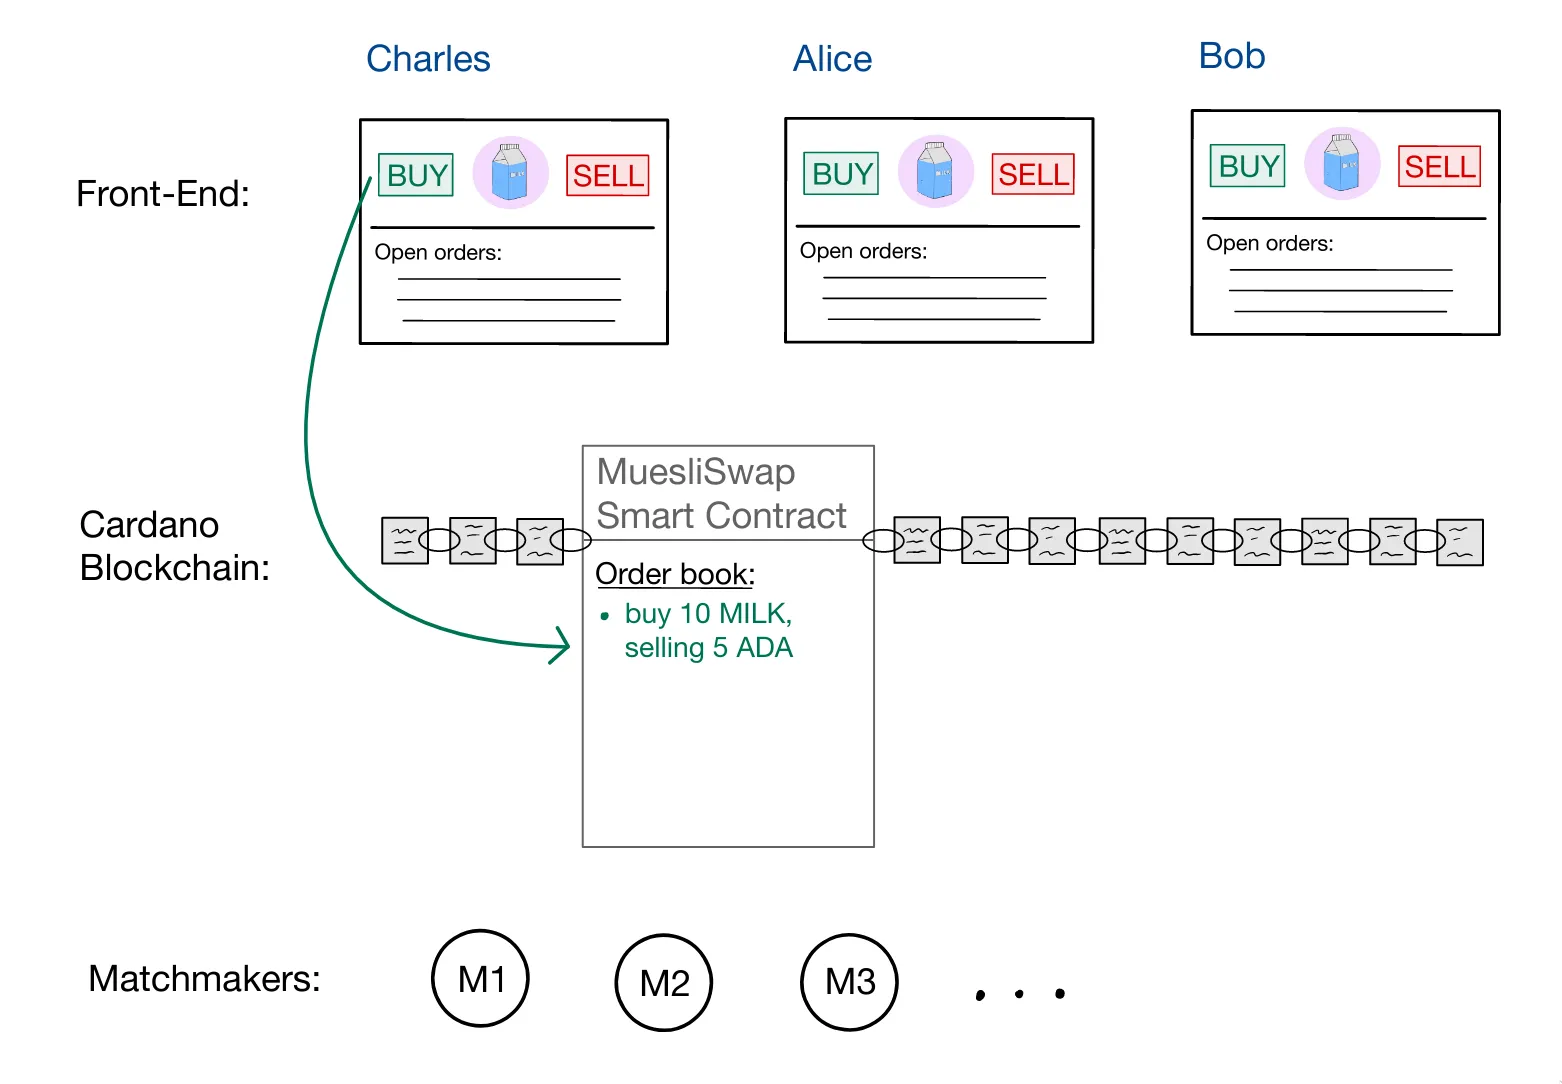
\includegraphics[scale=0.18]{illustration1.png}
    \caption{Alice and Bob joining the game by submitting competing orders. Which one might become matched with Charles’s?.}
    \label{fig:illustration2}
\end{figure}



\subsection{Matchmaking and Execution}
The matching of orders in the on-chain orderbook is facilitated by matchmakers—agents that scan the blockchain for new orders locked in the smart contract. When matchmakers identify two compatible orders, they initiate the exchange through the smart contract, which enforces the trade to be executed according to the specified terms, ensuring fairness and security. This process eliminates the need for a central coordinator, aligning with the principles of decentralization.

Matchmakers are incentivized through the profit margins left over from trades they facilitate. For instance, if a matchmaker matches Charles's order with Bob's, where Charles provided more ADA than needed, the matchmaker can keep the excess as a reward. This incentive mechanism encourages community participation in the matchmaking process, further decentralizing the operation of the exchange. For an illustration see \ref{fig:illustration3}

\begin{figure}[H]
    \centering
    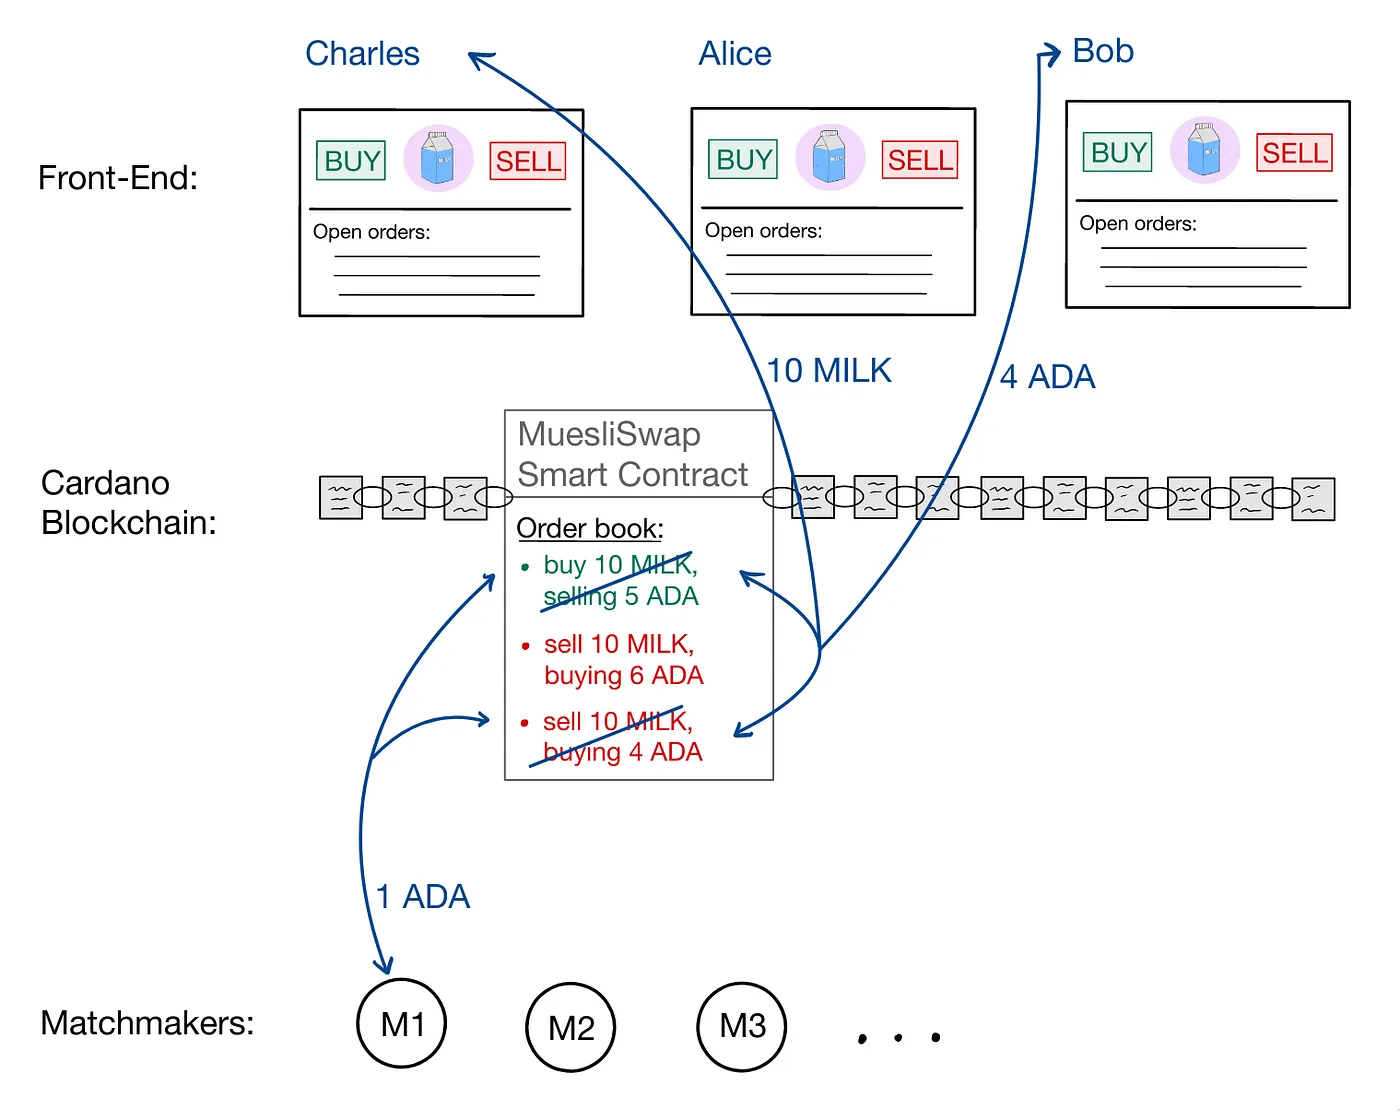
\includegraphics[scale=0.18]{illustration3.png}
    \caption{It's a match!}
    \label{fig:illustration3}
\end{figure}




\subsection{Decentralization} 
This smart contract protocol underscores the importance of true decentralization in its operations. By allowing traders to directly interact with a smart contract for order registration and execution, and distributing the task of order matching across the community, the protocol ensures that users' funds are managed transparently and securely. Moreover, the open nature of the platform means that anyone can become a matchmaker or develop their own interface for interacting with the protocol, fostering innovation and improving the trading experience.

\newpage
\section{Integration of DID into the MuesliSwap Orderbook Protocol}

This section outlines the conceptual integration of the Atala PRISM digital identity (DID) system into the MuesliSwap orderbook protocol, examining two distinct approaches to determine the most viable path for development. These approaches are evaluated based on their integration complexity for the orderbook model, focusing on the unique challenges and opportunities presented by the decentralized nature of MuesliSwap.

\subsection{Approach 1: Direct Integration through PRISM Protocol Transaction Parsing}

\paragraph{Design Concept.} The Atala PRISM framework facilitates the issuance of DIDs, which are recorded on the Cardano blockchain. A straightforward method to integrate user authentication within the MuesliSwap orderbook involves directly parsing these PRISM protocol transactions to validate a user's DID.

\paragraph{Orderbook Integration Challenges.} Integrating this approach into the MuesliSwap orderbook would necessitate the development of a mechanism for parsing PRISM transactions directly from the blockchain. This presents a significant challenge, particularly for ensuring that this process is compatible with the decentralized, smart contract-driven nature of the DEX. Additionally, the lack of a dedicated DID wallet for users to manage their identities introduces further complexity, necessitating the development of new infrastructure from the ground up.

\paragraph{On-chain Orderbook Authentication.} For a DEX like MuesliSwap, where trades are executed on-chain via smart contracts, validating DIDs on-chain is imperative. However, the complexity of parsing PRISM transactions within a Plutus smart contract poses substantial technical hurdles. Moreover, the necessity for a DID wallet remains, adding to the implementation challenge.

\paragraph{Conclusion.} The direct parsing approach is fraught with difficulties, especially for on-chain applications. Its lack of modularity—where authentication is tightly coupled with PRISM transactions within the smart contract—further complicates its practicality. Consequently, this approach is deemed unsuitable for the decentralized context of MuesliSwap, prompting consideration of an alternative strategy.

\subsection{Approach 2: Modular Authentication via NFTs}

\paragraph{Design Proposal.} A more flexible two-step authentication process is proposed:
\begin{enumerate}
\item Off-chain, users authenticate using their DID to mint an authentication Non-Fungible Token (NFT) that uniquely signifies their DID on the blockchain through its token metadata.
\item This authentication NFT is then used during trade transactions as proof of identity, mitigating the risk of fraudulent activities.
\end{enumerate}
This method benefits from the scalability of existing Atala PRISM-based identity solutions, such as ProofSpace, and the availability of established DID wallet technologies provided by these platforms.

\paragraph{Integration with MuesliSwap's Orderbook.} For MuesliSwap, the integration of authentication NFTs can streamline user verification processes without significant alterations to the existing trading mechanisms. During trade execution or order placement, users can prove their identity by associating their authentication NFT, thus ensuring a secure and compliant trading environment. In addition, if deemed necessary one could also require the DID authentication of the matchmaker matching orders. 

\paragraph{On-chain and Off-chain Flexibility.} This modular approach allows for seamless integration within both the on-chain order execution and off-chain order management processes of MuesliSwap. It leverages the blockchain's inherent security and transparency while enabling a user-friendly method for DID verification without the need for complex transaction parsing or bespoke wallet development.

\paragraph{Conclusion.} The modular nature of this approach, combined with the ability to incorporate existing DID solutions and wallet technologies, offers a robust and flexible framework for integrating digital identities into the MuesliSwap orderbook. This method not only aligns with the decentralized ethos of MuesliSwap but also enhances the platform's security, user trust, and regulatory compliance capabilities. Moving forward, this approach will be the focus of development efforts to integrate DIDs into the MuesliSwap ecosystem.

\newpage


\section{Smart contract specifications: DID Verification in the MuesliSwap Orderbook Protocol}

This section outlines the proposed design and functional integration of digital identity verification within the MuesliSwap Orderbook DEX, emphasizing the development of a smart contract infrastructure tailored to facilitate DID verification processes.

\paragraph{Modular Smart Contract Infrastructure.} At the core of integrating Atala PRISM DIDs into MuesliSwap is a modular smart contract infrastructure designed to enable secure and efficient verification of digital identities. This infrastructure consists of several key components, each with specific functionalities to support DID verification alongside trading activities on the orderbook.

\paragraph{Smart Contract Infrastructure for DID Verification.} The infrastructure will include:
\begin{itemize}
\item \textbf{Orderbook Contract:} Enhanced to incorporate DID verification results into the trading process. This contract will ensure that every order placed or fulfilled on the DEX is associated with a verified DID, enhancing the security and integrity of transactions.
\item \textbf{Authentication NFT Contract:} Facilitates the issuance of NFTs representing verified DIDs, allowing users to prove their identity on-chain efficiently. These NFTs will serve as a modular bridge between the off-chain DID verification process and on-chain trading activities.
\end{itemize}

\paragraph{Operational Requirements and Security Measures.} The system will be designed to ensure:
\begin{itemize}
\item \textbf{Inclusivity and Accessibility:} All NFT holders can participate in trading, with interfaces designed for ease of use, whether through manual contract interactions or user-friendly GUIs.
\item \textbf{Decentralization:} The process remains fully decentralized, preventing any single point of control over DID verification or trade authorization.
\item \textbf{Spam and Security Protections:} Implementations to prevent spam orders and enhance security, such as minimum token requirements for trade initiation and mechanisms to ensure the integrity of trade orders and DID verification outcomes.
\end{itemize}

\paragraph{Conclusion.} The proposed smart contract infrastructure and integration approach for incorporating DID verification within the MuesliSwap Orderbook DEX aims to enhance the platform's security, user trust, and compliance. By leveraging modular smart contracts for DID verification, MuesliSwap will set a new standard in decentralized trading, ensuring that all participants are verified and that their transactions are secure and transparent. 

\newpage
\section{Integration Plan for DID Verification in the MuesliSwap Orderbook}

MuesliSwap's orderbook platform revolutionizes decentralized trading on the Cardano blockchain, enabling users to engage in secure and direct token exchanges. The platform's optional extension to incorporate Atala PRISM digital identity (DID) verification represents a significant enhancement in security and regulatory compliance. This integration necessitates a strategic plan to seamlessly incorporate DID functionalities without disrupting the existing user experience.

\paragraph{Integration Strategy.} The core of our strategy is to develop a new "DID Verification Component" within the MuesliSwap ecosystem. This component will enable users to authenticate their identities through Atala PRISM DIDs, subsequently minting authentication Non-Fungible Tokens (NFTs) that represent their verified status on the blockchain. Given the distinct nature of incorporating on-chain DID verification within a primarily off-chain orderbook environment, our approach entails developing dedicated interfaces and backend processes that facilitate interaction with the Cardano blockchain, enhancing the platform's security and trustworthiness.

\paragraph{Technical Approach.} The integration involves several key steps:

\begin{itemize}
    \item User Interface Development: Crafting a new user interface tailored to the DID verification process. This interface will guide users through the process of DID authentication and authentication NFT minting, ensuring a seamless experience that aligns with MuesliSwap's existing UI/UX standards.
    \item Smart Contract Development: Designing and deploying smart contracts on the Cardano blockchain to handle the DID verification process, NFT minting, and integration with the orderbook trading mechanisms. These contracts will serve as the backbone of the new security layer, enabling verified trading activities.
    \item Backend Infrastructure: Establishing a new backend infrastructure that bridges the user interface with Cardano blockchain functionalities, including interactions with DID verification and authentication NFTs. This infrastructure will also support the retrieval of verified identities during the trading process, ensuring that all trades are conducted between authenticated parties.

\end{itemize}
\paragraph{Future Integration Possibilities.} While the initial phase focuses on establishing the foundational DID verification mechanisms, future developments may explore deeper integration possibilities. This could include native optional support for DID-based activities within the existing orderbook platform, further streamlining the user experience and expanding the platform's capabilities in secure, decentralized trading.

\end{document}
